%
% File:     chapter-schedule.tex
% Author:   awl8049
% Revision: $Revision: 1.2 $
%
\chapter{Thermal-Aware Scheduling}
\label{chp:schedule}
The current generation of operating systems treat the cores in a
multicore processor as distinct physical processors. Furthermore, the
advent of simultaneous multi-threading (such as Intel's HyperThreading
technology) has led to operating systems treating such virtualized
processors as equal ``logical CPUs'' that behave as independent
processors for scheduling purposes.  However, there are dependencies
between these logical CPUs that need to be taken into account when
balancing performance and energy efficiency.  These dependencies lead to
contention for shared resources which, in turn, leads to performance
penalties and inefficient use of energy.  The component of the operating
system most aware of the existence of multiple cores is the thread
scheduling algorithm.  The scheduler is responsible for ensuring that
all of the cores across all processors in a system is kept busy; the
scheduler must be able to efficiently migrate the state of threads
across processors regardless if that migration remains on a core or
across processors.

Modern multiprocessor operating systems such as Windows, Linux, Solaris,
and FreeBSD take a two-level approach to scheduling in an attempt to
maximize system resources.  The first level manages each core using a
distributed run queue model with per core queues and fair scheduling
policies. The second level attempts to balance the resource load by
redistributing tasks across the queues on each core.  The design of such
schedulers are based upon three principles: (1) threads are assumed to
be independent, (2) load is equated to queue length, and (3) locality is
important \cite{Hofmeyr2010}.

Traditional server load balancing makes assumptions about workload
behavior to make scheduling decisions.  Interactive workloads are
characterized by the independent tasks that remain quiet for extended
periods.  Server workloads contain large numbers of threads that are
highly independent of each other that use synchronization objects to
ensure mutual exclusion on small data items.  In parallel applications,
there is a higher levels of interaction between threads; consequently,
load balancing such applications requires additional mechanisms.  

Parallel applications are implemented most often on contemporary
processors using a Single Process, Multiple Data (SPMD) programming
model where logical CPUs simultaneously execute the same program at
independent points.  Tasks execute independently and communicate with
other nodes by sending and receiving messages with some form of barrier
synchronization implemented as part of the message interface.  The
details of the message process is isolated from the application by
standard interfaces such as MPI and OpenMP. %need cites!
Note how this programming model contravenes the assumptions for system
level load balancing: (1) threads are logically related, (2) have data
and control dependencies between threads, and (3) have equally long
life-spans \cite{Hofmeyr2010}.  

Our scheduler extends the existing dispatcher and power
management infrastructure in the operating system. It is the role of the
kernel thread scheduler to manage the placement of threads in a dispatch
queue, decide which thread to run on a processor, and manage the
movement of threads to and from processors so as to balance the workload
amongst logical CPUS.  A scheduler must fulfill this role while
addressing two major requirements for SPMD applications: (1) threads
composing an application must make equal progress and (2) the maximum
level of hardware parallelism is exploited.

However, these schemes do not take into account the increase in thermal
stress placed upon the processor entailed by focusing on maximum
performance.  Modern processors crudely manage this problem through Dynamic
Thermal Management (DTM) where the processor monitors the die
temperature and dynamically adjusts the processor voltage and frequency
(DVFS) to slow down the processor.  Prior work
\cite{Bircher2008,Donald2006,Coskun2008d} has shown that this technique has
significant negative impact on both performance and reliability in the
processor.   Thus, pro-active scheduling techniques that avoid thermal
emergencies are preferable to reactive hardware techniques such as DTM.

\section{Thread Selection}
\label{sec:whatnext}
The scheduler is responsible in each quantum for deciding which thread
to run on a processor.  We introduce in this work a heuristic scheduling
algorithm that reduces the thermal stress on a multicore processor
while addressing the SPMD requirements of equal progress and maximum
exploitation of parallelism.  The thermal predictor introduced in
Chapter~\ref{sec:themalmodel} is used to construct a on-line thermal
estimator for temperature, which is then used to predict which thread to
next execute on each logical CPU's run queue.

We enhance the existing thread infrastructure to maintain
the information required by the thermal estimator. Our implementation is
based upon the concept of Task Activity Vectors (TAVs) as introduced by 
\citeN{Merkel2008a}.  Each task maintains a vector with the required
history needed to make a prediction; in effect, we trade the additional
space required for keeping this history for the benefits gained from the
thermal scheduling.   At each scheduling quantum, each TAV is updated
with counts from the performance counters representing the hardware
resources used in the predictor.   The scheduler predicts the impact on
the logical CPU temperature using the thermal predictor to map the
PeCs values into an estimate of the ``thermal efficiency of
application'' (TEA) (as discussed in \ref{sec:themalmodel}).  

The predictions are then used by a policy-based heuristic predictor to
decide which thread to execute given the TEA of each candidate thread.
The operating system kernel is enhanced to allow the policy to be
selected as a kernel configuration option. We examine the behavior of
our predictor against three well known thermal scheduling heuristics:
(1) Greedy, (2) MinTemp \cite{Kursun2006}, and (3) ThreshHot
\cite{Zhou2010b}.  The Greedy heuristic selects the coolest job to
execute in each scheduling epoch, MinTemp selects the coolest possible
thread if over a set threshold, and ThreshHot selects the hottest thread
that is predicted to not cause the temperature to exceed that set
threshold or the hottest job in the queue otherwise.

\section{Load Balancing}
\label{sec:loadbalance}
Load balancing distributes workload evenly across the available logical
CPUs; current implementations distribute to maximize performance, we
enhance the concept to minimize thermal stress while seeking best
performance. We begin by organizing the logical CPUs in the system into
three categories based upon the temperature at which a DTM event occurs:
Hot (90\% of DTM temperature), warm (between 75\% and 90\% of DTM
temperature), and cold (less than 75\% of the DTM temperature).  In
addition, we classify each logical CPU into ``clans'' depending whether
a logical CPU is considered a ``fast processor'' or ``slow processor''
depending upon the current processor frequency of the underlying
hardware.  This two-level categorization allows us to manage the
distribution of work such that we can migrate work away from heat
sources while minimizing the impact on performance of threads.

The movement of logical CPUs between processor groups as temperature
increases is managed by a Thermal Predictor.  The Thermal Predictor
collect the values of the PeCs, temperature readings from the logical
CPUS, and utilization data from the dispatcher to decide whether a
processor will move towards the DTM temperature.  In this way we can
anticipate the DTM event and prevent its occurrence.

\begin{figure}[htbp]
  \centering
  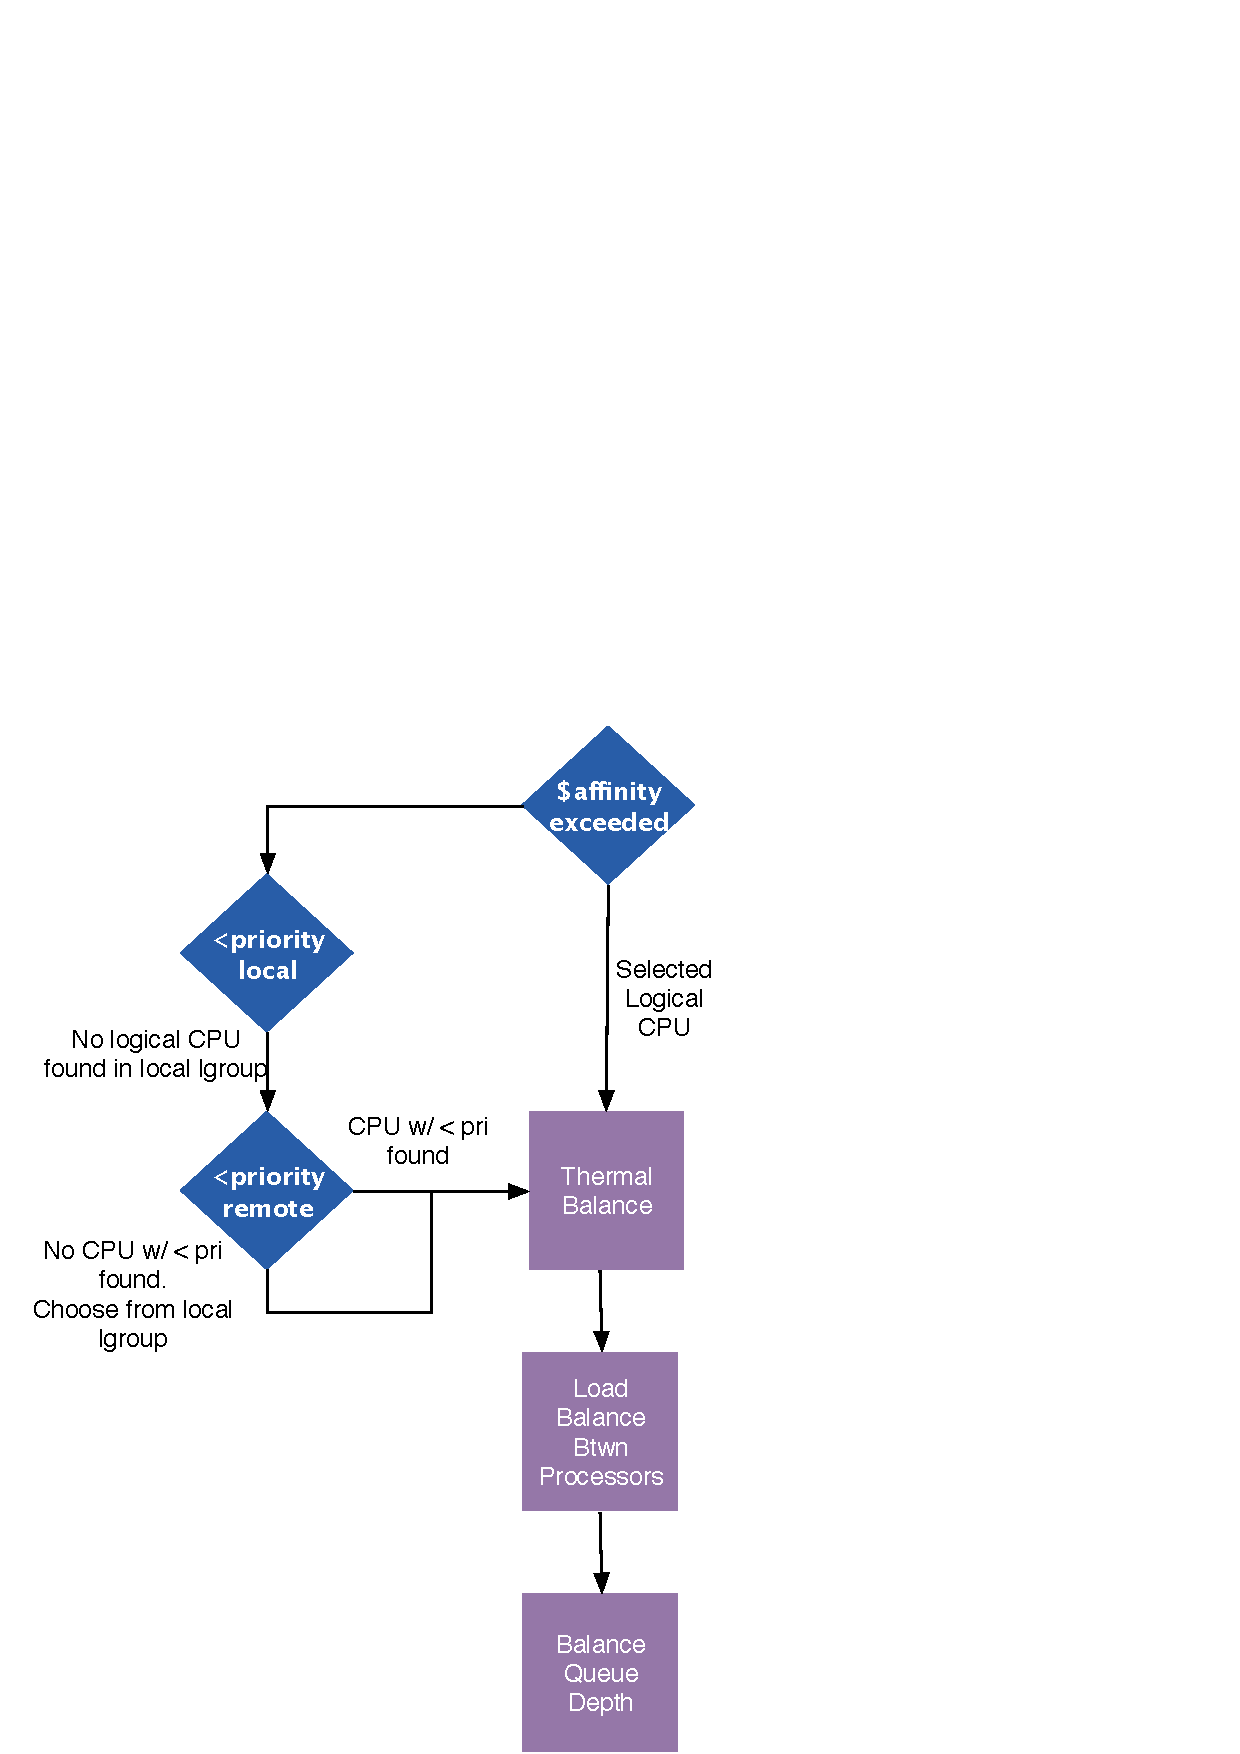
\includegraphics[scale=0.40]{threadinsert.pdf}
  \caption{Thread Queue Insertion}
  \label{fig:thread}
\end{figure}
The dispatcher is responsible for deciding where to insert threads into
run queues; i.e., when and where a thread will next execute. The steps
in this process are illustrated in Figure~\ref{fig:thread}.  First, the
dispatcher checks to see if the logical CPU where the thread was running
satisfies the cache affinity criteria (the default for OpenSolaris is
the thread was last running within the past 3 cycles).  If that test
fails, it tries to find the logical CPU in the local group running the
lowest priority thread.  If no thread is found in the local group, then
the dispatcher will check through known remote groups.  If no logical
CPU is found in either case, it will choose a logical CPU in the local
group.

At this point, the system will attempt to load balance the workload.
Two possibilities exist in the current system: equal balance across all
physical processors in the system and coalesce work onto one chip or the
other.  The first case is traditional example of load balancing while
the second case is attempting to free up as many resources as possible
to provide opportunities for power management to find logical units to
shut down.  We add a third sort of load balancing: temperature
balance. In this case, the dispatcher will attempt to load logical CPUs
in the ``COLD'' processor group first, followed by the ``WARM''
processor group, and finally the ``HOT'' group.

\subsection{Algorithm}
\label{sec:lbalgorithm}
Our Thermal-Aware Balancer (TAB) uses two classes of threads: a global
Thermal Predictor Thread (TPT) and multiple Thermal Balancing Threads
(TBT), one TBT per logical CPU.   The Thermal Predictor Thread is a
temperature monitor that watches the temperature of the logical CPU and
adjusts the HOT, WARM, COLD lists on a periodic basis.  The TBTs on each
logical CPU performs a mix of speed and thermal balancing
\cite{Hofmeyr2010} on queues assigned to each logical CPU.

The TPT awakes periodically and enumerates the known logical CPUs to
rearrange the HOT, WARM, COLD list.   The uses the thermal predictor
defined in the previous chapter to evaluate the past behavior of each
logical CPU and adds/deletes this unit from the appropriate
lists. 

\begin{lstlisting}[float,label=code:TABbalance,caption=TAB Balancing Algorithm]
begin
Determine if logical CPU is HOT, WARM, or COLD
if logical cpu is HOT
begin
   for each thread in the run queue
     begin
         Project the resulting change in temperature if this thread
         executes
         Compute the projected logical CPU speed over the elapsed balance
         interval
     end
   Compute the global core speed as average over all logical CPUs
   Migrate the thread with the ``worst'' impact on temperature to the
   logical CPU in the COLD set most suitable from a speed standpoint.
end
\end{lstlisting}
Periodically, the TBT on each core wakes up, check for imbalances
on the on the core and pulls threads from the hotter cores to local
cores and return to sleep.    Note that this is a distributed algorithm
where each TBT operates independently and without any global
synchronization.   A TBT executes the code in
Listing~\ref{code:TABbalance} when it awakes in order to adjust the
thermal balance of the queues in the designated logical CPU.


% Following comment block used by GNU-EMACS and AUCTEX packages
% Please do not remove.
%%% Local Variables: 
%%% mode: latex
%%% TeX-master: "prospectus.tex"
%%% End: 
